
\let\negmedspace\undefined
\let\negthickspace\undefined
\documentclass[journal,12pt,twocolumn]{IEEEtran}
\usepackage{cite}
\usepackage{amsmath,amssymb,amsfonts,amsthm}
\usepackage{algorithmic}
\usepackage{graphicx}
\usepackage{textcomp}
\usepackage{xcolor}
\usepackage{txfonts}
\usepackage{listings}
\usepackage{enumitem}
\usepackage{mathtools}
\usepackage{gensymb}
\usepackage[breaklinks=true]{hyperref}
\usepackage{tkz-euclide} 
\usepackage{listings}
\usepackage{gvv}
%
%\usepackage{setspace}
%\usepackage{gensymb}
%\doublespacing
%\singlespacing

%\usepackage{graphicx}
%\usepackage{amssymb}
%\usepackage{relsize}
%\usepackage[cmex10]{amsmath}
%\usepackage{amsthm}
%\interdisplaylinepenalty=2500
%\savesymbol{iint}
%\usepackage{txfonts}
%\restoresymbol{TXF}{iint}
%\usepackage{wasysym}
%\usepackage{amsthm}
%\usepackage{iithtlc}
%\usepackage{mathrsfs}
%\usepackage{txfonts}
%\usepackage{stfloats}
%\usepackage{bm}
%\usepackage{cite}
%\usepackage{cases}
%\usepackage{subfig}
%\usepackage{xtab}
%\usepackage{longtable}
%\usepackage{multirow}
%\usepackage{algorithm}
%\usepackage{algpseudocode}
%\usepackage{enumitem}
%\usepackage{mathtools}
%\usepackage{tikz}
%\usepackage{circuitikz}
%\usepackage{verbatim}
%\usepackage{tfrupee}
%\usepackage{stmaryrd}
%\usetkzobj{all}
%    \usepackage{color}                                            %%
%    \usepackage{array}                                            %%
%    \usepackage{longtable}                                        %%
%    \usepackage{calc}                                             %%
%    \usepackage{multirow}                                         %%
%    \usepackage{hhline}                                           %%
%    \usepackage{ifthen}                                           %%
  %optionally (for landscape tables embedded in another document): %%
%    \usepackage{lscape}     
%\usepackage{multicol}
%\usepackage{chngcntr}
%\usepackage{enumerate}

%\usepackage{wasysym}
%\documentclass[conference]{IEEEtran}
%\IEEEoverridecommandlockouts
% The preceding line is only needed to identify funding in the first footnote. If that is unneeded, please comment it out.

\newtheorem{theorem}{Theorem}[section]
\newtheorem{problem}{Problem}
\newtheorem{proposition}{Proposition}[section]
\newtheorem{lemma}{Lemma}[section]
\newtheorem{corollary}[theorem]{Corollary}
\newtheorem{example}{Example}[section]
\newtheorem{definition}[problem]{Definition}

\newcommand{\BEQA}{\begin{eqnarray}}
\newcommand{\EEQA}{\end{eqnarray}}
\newcommand{\define}{\stackrel{\triangle}{=}}
\theoremstyle{remark}
\newtheorem{rem}{Remark}


\begin{document}


\bibliographystyle{IEEEtran}


\vspace{3cm}

\title{
	Question 1.5.9
}

\author{
	EE22BTECH11054 - Umair Parwez
}	

\maketitle
\newpage
\bigskip

\renewcommand{\thefigure}{\theenumi}
\renewcommand{\thetable}{\theenumi}

\begin{flushleft}
	\textbf{Question 1.5.9}\\
	\bigskip
	Given triangle ABC with vertices, 
	\begin{align}
		\vec{A} = \myvec{1\\ -1}, \vec{B} = \myvec{-4\\ 6}, \vec{C} = \myvec{-3\\ -5}
	\end{align}\\
	find the points of contact, $\vec{E}_3$ and $\vec{F}_3$, of the incircle with sides AC and AB respectively.\\
	\bigskip
\end{flushleft}

\begin{flushleft}
	\textbf{Solution}\\
	\bigskip

	Required to find points of contact, $\vec{E}_3$ and $\vec{F}_3$, of incircle with sides AC and AB respectively.\\

	\bigskip

	From previous questions we know the coordinates of the incircle are : 
	\begin{align}
		\vec{I} = 
		\myvec {
			\frac{-53-11\sqrt{37}+7\sqrt{61}+\sqrt{2257}}{12} \\ \\
			\frac{5-\sqrt{37}+5\sqrt{61}-\sqrt{2257}}{12}
		}
	\end{align}\\

	Radius of incircle is :
    \begin{align}
		r = \frac{185+41\sqrt{37}-37\sqrt{61}-\sqrt{2257}}{6\sqrt{74}}
    \end{align}\\

	Equation of incircle is : 
	\begin{align}
		{\norm{ \vec{x}-\vec{I} }}^2 = {r}^2 
	\end{align}\\

	points $\vec{A}$, $\vec{B}$ and $\vec{C}$ are : 
	\begin{align}
		\vec{A} = \myvec{
			1\\
			-1
		}, 
		\vec{B} = \myvec{
			-4\\
			6
		}, 
		\vec{C} = \myvec{
			-3\\
			-5
		}
	\end{align}\\

	Parametric equation of AC is :
	\begin{align}
		\vec{x} = \vec{A} + k(\vec{A}-\vec{C})
	\end{align}\\
	
	Substituting (5) in (3) : 
	\begin{align}
		{\norm{ \vec{A}+k(\vec{A}-\vec{C})-\vec{I} }}^2 = {r}^2 
	\end{align}
	\begin{align}
		(\vec{A}+k(\vec{A}-\vec{C})-\vec{I})\cdot(\vec{A}+k(\vec{A}-\vec{C})-\vec{I}) = {r}^2
	\end{align}
	\begin{align}
		k^2 \norm{\vec{A}-\vec{C}}^2 + 2k(\norm{\vec{A}}^2 - {\vec{A}}^T \vec{C} - {\vec{I}}^T \vec{A} + {\vec{I}}^T \vec{C}) + \norm{\vec{A}-\vec{I}}^2 = {r}^2
	\end{align}

	Since AC is tangent to the incircle, the discriminant of the obtained quadratic equation is zero and the value of k is given as :

	\begin{align}
		k = -\frac{(\norm{\vec{A}}^2 - {\vec{A}}^T \vec{C} - {\vec{I}}^T \vec{A} + {\vec{I}}^T \vec{C})}{\norm{\vec{A}-\vec{C}}^2}
	\end{align}\\

	Upon substituting the values of $\vec{A}$, $\vec{C}$ and $\vec{I}$ into (10) we get,  
	\begin{align}
		k = \frac{-4-\sqrt{37}+\sqrt{61}}{2}
	\end{align}\\

	Substituting (11) back into (5), we get point of contact with AC,
	\begin{align}
		\vec{E}_3 = \myvec{
			\frac{-2-\sqrt{37}+\sqrt{61}}{2}\\ \\
			\frac{-6-\sqrt{37}+\sqrt{61}}{2}
		}
	\end{align}\\

	\bigskip
	Now let us find the other point of contact, with AB.\\
	\bigskip
	Parametric equation of AB is : 
	\begin{align}
		x = \vec{A} + k(\vec{A}-\vec{B})
	\end{align}\\

	We can get the value of k by replacing $\vec{C}$ with $\vec{B}$ in Eq(10). Upon substituting the values, we get, 

	\begin{align}
		k = \frac{-37-4\sqrt{37}+\sqrt{2257}}{74}
	\end{align}\\

	Substituting (14) back into (13), we get point of contact with AB,
	\begin{align}
		\vec{F}_3 = \myvec{
			\frac{-111-20\sqrt{37}+5\sqrt{2257}}{74}\\ \\
			\frac{185+28\sqrt{37}-\sqrt{2257}}{74}
		}
	\end{align}\\
	
	\bigskip

	Diagram is shown on next page.

\end{flushleft}

\newpage

\begin{figure}[h]
	\centering
	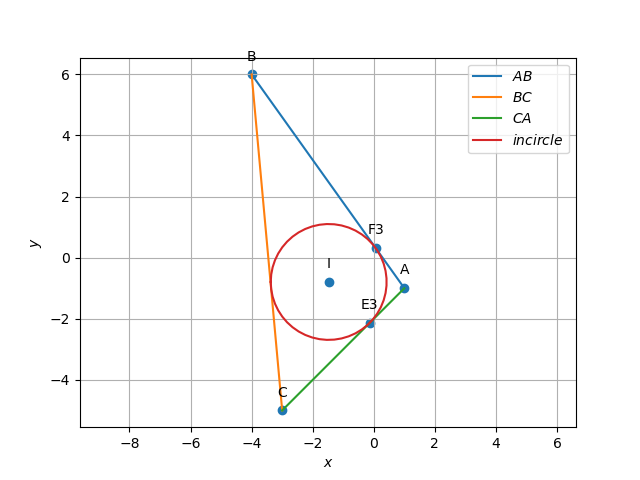
\includegraphics[width=\columnwidth]{./figs/Diagram.png}
	\caption{Points of contact of incircle}
	\label{Incircle}
\end{figure}

\end{document}


